\documentclass{zc-ust-hw}

\usepackage{lipsum}
\usepackage[]{caption} 
\usepackage[]{subcaption} 
\usepackage[]{pgfplots}

\newcommand*{\name}{
  Amr Khaled (202200809),
  Ashar Salama (202200199),
  \\ \hspace*{4.63em}
  Asser Khaled (202201340),
  Eyad Alaa-eldin (202200103),
  \\ \hspace*{4.63em}
  SalahDin Ahmed (202201079)
}
\newcommand*{\course}{Thermodynamics, Wave Motion and Optics (PHYS201)}
\newcommand*{\assignment}{Participation 3}

\begin{document}

\maketitle

\begin{enumerate}
  \item Suppose you are given two mirrors paced at $90^\circ$ to each other as shown
    the in figure. Use the ray methodology to find out the images formed of the
    red arrow due to this mirror system. Note: the images formed does not
    depend on the place of the observer.

    \begin{figure}[htpb]
      \centering
      \includegraphics[width=0.8\textwidth]{figures/light-reflection.png}
      \caption{Light reflection.}
      \label{fig:light-reflection-png}
    \end{figure}

    \newpage

  \item For the case of the phenomena of multiple reflections and images formed
    in a system of two plane mirrors, Derive a formula for the number of images
    formed as a function of the angle between the two mirrors. You may make use
    of the experimental data provided in the lecture for the number of images
    formed at different angles.

    \begin{figure}[htpb]
      \centering
      \begin{subfigure}{0.45\textwidth}
        \centering
        \includegraphics[width=\linewidth]{figures/90.png}
        \caption{$\theta=90^\circ$}
        \label{fig:sub1}
      \end{subfigure}
      \hfill
      \begin{subfigure}{0.45\textwidth}
        \centering
        \includegraphics[width=\linewidth]{figures/60.png}
        \caption{$\theta=60^\circ$}
        \label{fig:sub2}
      \end{subfigure}

      \medskip

      \begin{subfigure}{0.45\textwidth}
        \centering
        \includegraphics[width=\linewidth]{figures/45.png}
        \caption{$\theta=45^\circ$}
        \label{fig:sub3}
      \end{subfigure}
      \hfill
      \begin{subfigure}{0.45\textwidth}
        \centering
        \includegraphics[width=\linewidth]{figures/30.png}
        \caption{$\theta=30^\circ$}
        \label{fig:sub4}
      \end{subfigure}

      \caption{Images formed at different angles.}
      \label{fig:images}
    \end{figure}

    \newpage

    \begin{figure}[t]
      \begin{minipage}{0.5\textwidth}  % Adjust the width as needed
        \centering
        \begin{tabular}{|c|c|}
          \hline
          $\theta$ & \# \\
          \hline
          90$^\circ$ & 3 \\
          \hline
          60$^\circ$ & 5 \\
          \hline
          45$^\circ$ & 7 \\
          \hline
          30$^\circ$ & 11 \\
          \hline
        \end{tabular}
        \captionof{table}{Number of images formed at different angles.}
        \label{tab:no-angle}
      \end{minipage}%
      \begin{minipage}{0.5\textwidth}  % Adjust the width as needed
        \centering
        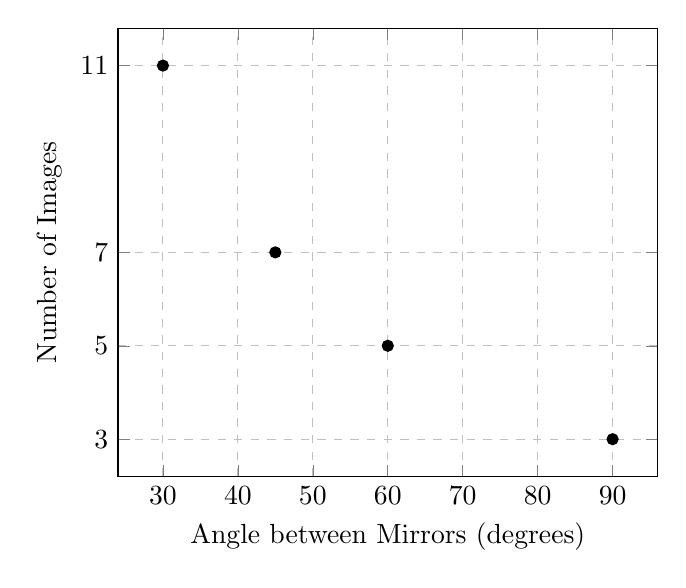
\begin{tikzpicture}[scale=1, transform shape]
          \begin{axis}[
            xlabel={Angle between Mirrors (degrees)},
            ylabel={Number of Images},
            legend pos=north west,
            grid=both,
            grid style=dashed,
            ytick={3, 5, 7, 11},
            ]
            \addplot[only marks] coordinates {
                (30, 11)
                (45, 7)
                (60, 5)
                (90, 3)
                % Add more experimental data points as needed
              };
          \end{axis}
        \end{tikzpicture}
        \caption{Plot of Table~\ref{tab:no-angle}.}
        \label{fig:plot}
      \end{minipage}
    \end{figure}

    From Figure~\ref{fig:plot} and Table~\ref{tab:no-angle}:
    \begin{align}
      \# &\propto \frac{1}{\theta} \\
      \# &= \frac{m}{\theta} + c
    .\end{align}
    Using linear regression:
    \begin{align}
      m = \frac{\Sigma y \Sigma x^2-\Sigma y \Sigma xy}{n\left( \Sigma x^2 \right) - \left( \Sigma x \right)^2 } &\quad
      c = \frac{n\left( \Sigma xy \right) - \Sigma x\Sigma y}{n\left( \Sigma x^2 \right) - \Sigma x^2 } \\
      m = 360 &\quad c = -1
    .\end{align}
    \begin{align}
      \# &= \frac{360}{\theta} - 1 \label{eq:final}
    .\end{align}

    \begin{figure}[htpb]
      \centering
      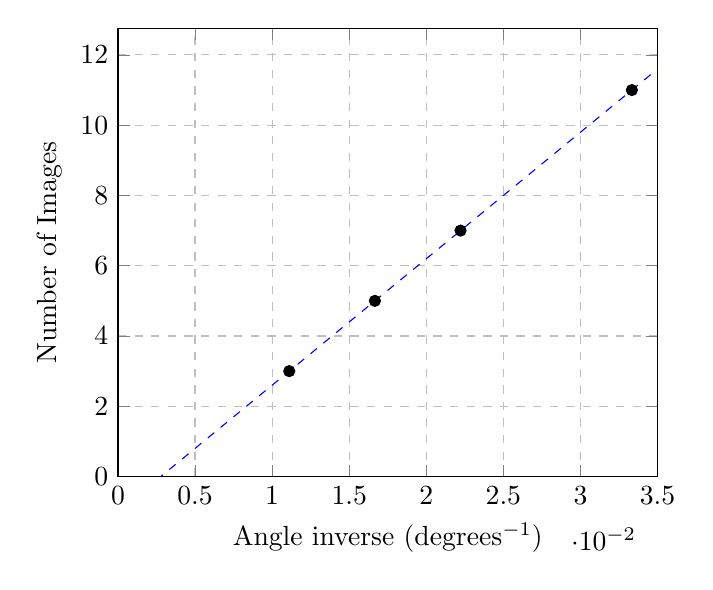
\begin{tikzpicture}
        \begin{axis}[
          xlabel={Angle inverse (degrees$^{-1}$)},
          ylabel={Number of Images},
          legend pos=north west,
          grid=both,
          grid style=dashed,
          ymin=0,
          xmin=0, xmax=0.035,
          % ytick={3, 5, 7, 11},
          % xtick={1/30, 1/45, 1/60, 1/90},
          ]
          \addplot[only marks] coordinates {
              (1/30, 11)
              (1/45, 7)
              (1/60, 5)
              (1/90, 3)
              % Add more experimental data points as needed
            };
          % Equation
          \addplot[domain=0:0.035, samples=100, color=blue, style=dashed]{360*x-1};
        \end{axis}
      \end{tikzpicture}
      \caption{Plot of Table~\ref{tab:no-angle} with Equation~\ref{eq:final}.}
      \label{fig:plot-equation}
    \end{figure}

\end{enumerate}

\end{document}
